\chapter{Case studies and experiment}\label{chap5}

\section{Field Study at E4C Charging Stations}
To ground the digital twin in real-world conditions, I conducted a field study at the \textbf{E4C campus charging stations}.  
During this visit, I collected operational datasets covering the period \textbf{2023–2025}.  
The dataset contained detailed records of charging activities, including session start times, durations, energy consumption, and connector usage.  
This empirical foundation ensured that the system was not only tested with synthetic data but validated against actual infrastructure behavior.

\section{Data Cleaning and Preprocessing}
The raw dataset required significant preparation before being used to create NGSI-LD entities.  
Using \textbf{Python}, I performed the following steps:
\begin{itemize}
    \item Removed incomplete or corrupted records,
    \item Standardized time formats and attribute naming conventions,
    \item Corrected missing or inconsistent values,
    \item Structured the dataset into NGSI-LD compliant JSON payloads.
\end{itemize}

This preprocessing ensured semantic consistency and made the data suitable for integration with the FIWARE ecosystem.

\section{Entity Creation}
Based on the cleaned dataset, I instantiated the NGSI-LD data model by creating entities and publishing them to the Orion Context Broker.  
The final set of entities included:
\begin{itemize}
    \item \textbf{1 \texttt{ChargingStation}} entity, representing the physical E4C charging facility,
    \item \textbf{1 \texttt{ChargingPoint}} entity, corresponding to the charging connector in use,
    \item \textbf{1 \texttt{EV}} entity, representing the electric vehicle interacting with the infrastructure,
    \item \textbf{2,200 \texttt{ChargingSession}} entities, each capturing the temporal and operational details of individual charging events.
\end{itemize}

These entities were distributed across MongoDB (for the latest state) and CrateDB (for historical time-series records), ensuring both real-time context management and analytical capabilities.  

\section{Summary}
By combining on-site observations, real data collection, rigorous preprocessing, and automated entity creation, the experimen

Define and Initialize the 3 scenarios
result of real data (cite some Kristian's work)
result of fake data
\section{Simulation Scenarios}

In addition to the real dataset collected from the E4C charging stations, I also designed synthetic experiments to evaluate the flexibility of the digital twin system under different user behavior assumptions.  
Three charging start-time scenarios were simulated, as illustrated in Figure~\ref{fig:charging_scenarios}.

\begin{figure}[ht!]
    \centering
    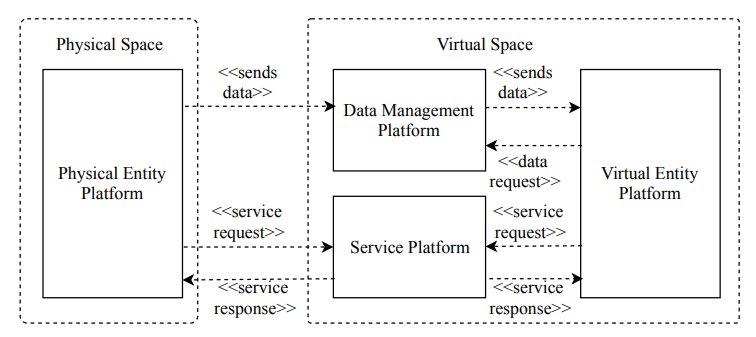
\includegraphics[width=0.9\textwidth]{Images/DT_diagram.png}
    \caption{Three charging scenarios simulated within the digital twin}
    \label{fig:charging_scenarios}
\end{figure}

\subsection*{Scenario 1: Random Time}
In this scenario, charging sessions were generated at completely random moments within the year:
\begin{itemize}
    \item Days $\in [0,364]$, 
    \item Hours $\in [0,23]$, 
    \item Minutes $\in [0,59]$, 
    \item Seconds $\in [0,59]$. 
\end{itemize}

\textbf{Rationale:} This represents uncontrolled charging behavior, where users connect their vehicles without considering price signals, grid conditions, or time of day.  
It serves as a \emph{baseline scenario} to evaluate the system under maximum randomness.

\subsection*{Scenario 2: Slot Time}
In this scenario, charging sessions follow a probability distribution across four time slots:
\begin{itemize}
    \item Morning (7:00–11:00): 20\%,
    \item Daytime (11:00–18:00): 30\%,
    \item Evening (18:00–22:00): 20\%,
    \item Night (22:00–7:00): 30\%.
\end{itemize}

\textbf{Rationale:} This reflects typical mobility and charging patterns observed in practice:  
drivers often charge after commuting in the morning or evening, or leave vehicles plugged in overnight.  
It provides a more realistic scenario compared to purely random charging.

\subsection*{Scenario 3: Informed Time}
In this scenario, user decisions are influenced by external factors such as dynamic electricity prices or demand-response programs:
\begin{itemize}
    \item 60\% of sessions occur during \textbf{off-peak hours} (10:00–16:00), modeled with a normal distribution,
    \item 40\% of sessions are distributed randomly across all other times.
\end{itemize}

\textbf{Rationale:} This simulates \emph{smart charging strategies}, where users or automated systems shift demand to off-peak hours.  
It illustrates how incentives and grid-awareness can reduce stress on the electricity network and improve overall efficiency.

\subsection*{Summary}
The three scenarios—\textbf{random}, \textbf{slot-based}, and \textbf{informed}—were designed to capture a spectrum of charging behaviors: from uncontrolled, to realistic, to optimized.  
By testing the digital twin under these conditions, I could assess whether the backend and visualization pipeline remained consistent and scalable across different user behavior models.

\section{Analysis of Real Data and Generation of Synthetic Sessions}

To ensure that the digital twin was both grounded in reality and capable of supporting simulation, I worked with two complementary datasets: the \textbf{real charging sessions} collected from the E4C stations and the \textbf{synthetic sessions} generated under controlled scenarios.

\subsection*{Analysis of Real Historic Data}
The real dataset contained approximately \textbf{4,400 charging session records} from 2023–2025.  
A statistical analysis was conducted to extract key characteristics:

\begin{itemize}
    \item The \textbf{mean session duration} was approximately \textbf{225.9 minutes}.
    \item The \textbf{mean energy consumption} was approximately \textbf{15.9 kWh}.
    \item Boxplot analysis revealed that successful sessions (\texttt{ended}) had diverse durations and consumption levels, whereas failed sessions (\texttt{failed}) were typically very short with negligible energy use.
\end{itemize}

A linear regression confirmed the strong correlation between duration and energy consumption:
\[
    \text{consumption} = 0.0557 \times \text{duration} + 3.3513
\]
This model indicated that longer sessions consume proportionally more energy, with a baseline offset due to fixed overhead.

\begin{figure}[ht!]
    \centering
    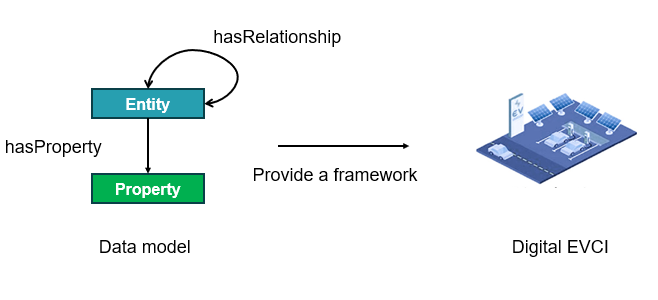
\includegraphics[width=0.95\textwidth]{Images/data-model.png}
    \caption{Analysis of real charging session data: duration distribution, consumption distribution, and duration–consumption correlation.}
    \label{fig:real_data_analysis}
\end{figure}

\subsection*{Generation of Synthetic Charging Sessions}
Based on the insights from the real dataset, I generated synthetic \texttt{ChargingSession} entities for the three charging scenarios (random, slot-based, informed).  
When creating these entities, the following measures were taken to preserve realism:

\begin{itemize}
    \item \textbf{Temporal distribution:} Session start times followed the probability rules defined by the three scenarios.
    \item \textbf{Durations:} Session lengths were sampled from distributions calibrated against the real data.
    \item \textbf{Energy consumption:} For each synthetic session, the value was derived using the regression model, ensuring consistency between duration and consumption.
\end{itemize}

This process resulted in thousands of synthetic sessions that shared the same statistical properties as the real dataset, while allowing controlled experiments under different charging behavior assumptions.  
The combination of empirical grounding and simulated flexibility validated the robustness of the digital twin architecture.

\section{Performance Evaluation}

To evaluate the responsiveness of the system, I tested the performance of three basic NGSI-LD operations: \textbf{create}, \textbf{update}, and \textbf{delete}.  
Each test was executed 20 times, and the response times were recorded.  
The results are summarized in Table~\ref{tab:performance}.

\begin{table}[ht!]
    \centering
    \caption{Performance evaluation of NGSI-LD operations (20 iterations each)}
    \label{tab:performance}
    \begin{tabular}{|l|c|c|c|c|c|}
        \hline
        \textbf{Operation} & \textbf{Success rate} & \textbf{Min (ms)} & \textbf{Max (ms)} & \textbf{Average (ms)} & \textbf{Median (ms)} \\
        \hline
        Create  & 100\% (20/20) & 10.3 & 27.5 & 17.5 & 18.4 \\
        \hline
        Update  & 100\% (20/20) & 10.6 & 20.1 & 16.4 & 18.3 \\
        \hline
        Delete  & 100\% (20/20) & 10.6 & 20.3 & 13.7 & 13.0 \\
        \hline
    \end{tabular}
\end{table}

\subsection*{Analysis}
The results show that all three operations achieved a \textbf{100\% success rate} with no failures.  
Response times were consistently low across all operations:
\begin{itemize}
    \item \textbf{Create} operations averaged 17.5 ms,
    \item \textbf{Update} operations averaged 16.4 ms,
    \item \textbf{Delete} operations averaged 13.7 ms.
\end{itemize}

These results demonstrate that the backend architecture provides fast and reliable entity management, even when handling multiple iterations of create, update, and delete requests.


\section{Frontend Visualization with Grafana}

To provide an intuitive interface for exploring the data stored in CrateDB, I integrated \textbf{Grafana} as the visualization layer of the digital twin.  
Grafana allowed me to design interactive dashboards that display the temporal evolution of charging activities and energy consumption.

\subsection*{Bar Chart Visualization}
One of the main visualizations I implemented was a series of \textbf{bar charts} showing the variation of energy consumption over time.  
These charts provided a clear overview of charging demand across different periods and allowed comparisons between usage patterns.

\subsection*{Interactive Features}
The Grafana dashboards were designed to be fully interactive:
\begin{itemize}
    \item \textbf{Time selection:} Users can choose any custom time window (daily, weekly, monthly) to observe energy consumption trends.
    \item \textbf{Charging point selection:} The dashboard includes filters that allow users to focus on a specific charging point or aggregate multiple points for comparison.
    \item \textbf{Dynamic queries:} All charts are powered by SQL queries to CrateDB, ensuring that data is updated in real time as new sessions are ingested.
\end{itemize}

\subsection*{Added Value}
By combining these features, the Grafana dashboards enabled:
\begin{itemize}
    \item Quick identification of peak demand hours,
    \item Analysis of charging point utilization levels,
    \item Better understanding of long-term energy consumption patterns.
\end{itemize}

\begin{figure}[ht!]
    \centering
    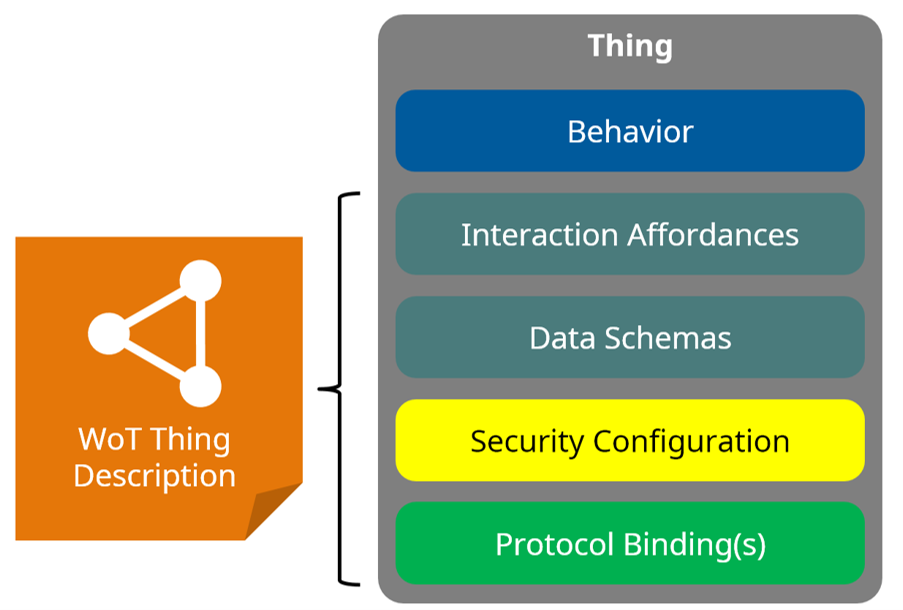
\includegraphics[width=0.9\textwidth]{Images/td.png}
    \caption{Example Grafana dashboard: energy consumption variation over time, with interactive selection of time windows and charging points.}
    \label{fig:grafana_dashboard}
\end{figure}

\subsection*{Summary}
The integration of Grafana completed the digital twin pipeline by turning raw and historical data into actionable insights.  
Through interactive dashboards, stakeholders can now monitor charging activity, analyze energy demand, and explore infrastructure usage patterns in real time.

% \textbf{Insérer une liste~:}
% \begin{itemize}
%     \item Premier niveau
%     \begin{itemize}
%         \item[(i)] Deuxième niveau
%         \item[(ii)] Un autre élément au deuxième niveau
%     \end{itemize}
%     \item Un autre élément au premier niveau
%         \begin{itemize}
%         \item[(a)] Deuxième niveau
%         \item[(b)] Un autre élément au deuxième niveau
%     \end{itemize}
% \end{itemize}
% \bigskip

% \textbf{Insérer un tableau simple~:} 
% \begin{table}[H]
%     \centering
%     \begin{tabular}{|c|c|c|c|c|c|c|c|c|c|}
%         \hline
%         A & B & C & D & E & F & G & H & I & \dots \\
%         \hline
%         1 & 2 & 3 & 4 & 5 & 6 & 7 & 8 & 9 & \dots\\
%         10 & 11 & 12 & 13 & 14 & 15 & 16 & 17 & 18 & \dots \\
%         \hline
%     \end{tabular}
%     \caption{\textbf{Titre.} \lipsum[1][1-3]}
%     \label{tab:table-label}
% \end{table}

% \textbf{Autre style de tableau~:} 
% \begin{table}[H]
%     \centering
%     \begin{tabular}{c c c c c}
%         \hline
%         \textbf{Col1} & \textbf{Col2} & \textbf{Col3} & \textbf{Col4} & \textbf{Col5} \\
%         \hline
%         1 & 2 & 3 & 4 & 5 \\
%         1 & 2 & 3 & 4 & 5 \\
%         \hline
%     \end{tabular}
%     \caption{\textbf{Titre.} \lipsum[1][1-3]}
%     \label{tab:table-label}
% \end{table}


% \section{Insertion de code Python}
% \textbf{Insérer du code en \textit{inline}~:} \texttt{print("Hello, World!")}.\\


% \textbf{Insérer du code en \textit{inline} avec coloration syntaxique~:} \mintinline{python}{print("Hello, World!")}.\\

% \textbf{Insérer du code en bloc avec coloration syntaxique~:} 
% \begin{minted}[bgcolor=codebg,fontsize=\small,frame=lines,linenos]{python}
% def factorial(n):
%     if n == 0:
%         return 1
%     else:
%         return n * factorial(n - 1)

% # Example usage
% print(factorial(5))  # Output: 120
% \end{minted}



% \section{Expressions mathématiques}
% \subsection{Théorèmes, propositions, définitions, lemmes, demonstrations...}

% \begin{theorem}
%     \lipsum[1][1-4]
% \end{theorem}

% \begin{proof}
%     \lipsum[1][1-4]
% \end{proof}

% \begin{proposition}
%     \lipsum[1][1-4]
% \end{proposition}

% \begin{definition}
%     \lipsum[1][1-4]
% \end{definition}

% \begin{remark}
%     \lipsum[1][1-4]
% \end{remark}

% \begin{lemma}
%     \lipsum[1][1-4]
% \end{lemma}


% \subsection{Equations et calculs sur plusieurs lignes}

% \subsubsection*{Une simple équation}
% \begin{equation}
%     e = mc^2
% \end{equation}

% \subsubsection*{Une équation sur plusieurs lignes}
% \begin{equation}
%     \begin{split}
%         \mathbb{E}(aX + Y) &= \mathbb{E}(aX) + Y\\
%                            &= a\mathbb{E}(X) + Y
%     \end{split}
% \end{equation}

% \subsubsection*{Une équation avec plusieurs cas}
% \begin{equation}
%     u_n =
%     \begin{cases}
%         1 \text{ if } n\equiv0 \mod 2\\
%         0 \text{ if } n\equiv1 \mod 2 \\
%     \end{cases}
% \end{equation}

% \subsubsection*{Insérer une série de calculs}
% \begin{align*}
%     x &= 0.999\ldots \\
%     10x &= 9.999\ldots \\
%     10x - x &= 9.999\ldots - 0.999\ldots \\
%     9x &= 9 \\
%     x &= 1 \\
%     0.999\ldots &= 1
% \end{align*}

% \subsection{Utilisation du glossaire}

% \newglossaryentry{esperance}{
%     name=espérance,
%     description={Valeur moyenne théorique d'une variable aléatoire}
% }


% Référence au glossaire : \gls{esperance}.  




